\chapter{Activity Equation in Python: decay class}
\label{section:decayclass}

\section{Full Source Code}

The full source code is available to download from github.

https://github.com/BenPalmer1983/atomic\_dictionaries

https://github.com/BenPalmer1983/decay



\section{Highlighted Code}

The code below is taken from the decay class and it is specifically responsible for calculating the amount of isotopes in the decay chain at some time t.

\lstinputlisting[style=sPython,caption={Decay python3 class for calculating the amount of an isotope in a decay chain at time t}]{appendix/activity_equation/decay.py}






\FloatBarrier
\clearpage

\section{Activity Equation Testing}
\subsection{Numeric Fortran Code}
\label{section:decaypo216numeric}

A simple Fortran code was created for each decay path used to test the activity equation and computer code.  The version of the code used to calculate the amount of each isotope for the Po-216 decay chain is given in fig. \ref{lst:decaypo216fortran}, and this code was modified for each decay chain tested.

\lstinputlisting[style=sBash,caption={Bash file to compile Fortran test code},label={lst:decaypo216make}]{appendix/activity_equation/make.sh}

\lstinputlisting[style=sFortran,caption={Fortran code to numerically estimate the amount of each isotope in the Polonium-216 decay chain},label={lst:decaypo216fortran}]{appendix/activity_equation/main.f90}

\clearpage
\subsection{Chromium-49}
\FloatBarrier

Chromium-49 has a straightforward decay path, via positron emission (or electron capture) through to Vanadium-49 then to the stable isotope Titanium-49.  Calculated isotope amounts are given for 5 different trial source rates and starting amounts; the results are listed in table \ref{table:cr49trialdata}.  The \acrshort{rss} error between the numeric and analytic code in this decay chain over all five trials was $6.52 \times 10^{-3}$ and the total percentage error between the two was $2.17 \times 10^{-3}\%$.

\begin{figure}[!h]
\centering
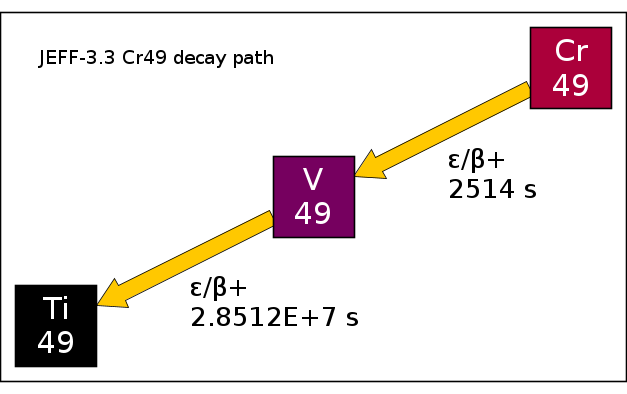
\includegraphics[width=.4\linewidth]{appendix/activity_equation/decay_paths/24cr49_decay.png}
\caption{Decay path for Chromium-49 \cite{jeff311}}
\label{fig:decaycr49}
\end{figure}

\FloatBarrier


\begin{table}[h]
\begin{center}
\begin{longtable}{c c c c c c c}
\hline\hline
 &  & Trial 1 & Trial 2 & Trial 3 & Trial 4 & Trial 5 \\
\hline\hline
${}^{49}_{24}Cr$ & $\omega$ & 
${0.0} \times 10^{0}$ & ${1.0} \times 10^{2}$ & ${0.0} \times 10^{0}$ &
${2.5} \times 10^{0}$ & ${2.5} \times 10^{0}$ \\
 & $n_{\text{start}}$ & 
${0.0} \times 10^{0}$ & ${0.0} \times 10^{0}$ & ${1.0} \times 10^{2}$ & 
${3.0} \times 10^{4}$ & ${3.0} \times 10^{4}$ \\
Numeric & $n_{\text{end}}$ & 
${0.0} \times 10^{0}$ & ${3.62694} \times 10^{5}$ & ${4.51169} \times 10^{-9}$ & 
${9.06734} \times 10^{3}$ & ${9.06734} \times 10^{3}$ \\
Analytic & $n_{\text{end}}$ & 
${0.0} \times 10^{0}$ & ${3.62694} \times 10^{5}$ & ${4.51169} \times 10^{-9}$ & 
${9.06734} \times 10^{3}$ & ${9.06734} \times 10^{3}$ \\
\hline
${}^{49}_{23}V$ & $\omega$ & 
${0.0} \times 10^{0}$ & ${0.0} \times 10^{0}$ & ${0.0} \times 10^{0}$ &
${0.0} \times 10^{0}$ & ${1.07} \times 10^{0}$ \\
 & $n_{\text{start}}$ & 
${0.0} \times 10^{0}$ & ${0.0} \times 10^{0}$ & ${0.0} \times 10^{0}$ &
${0.0} \times 10^{0}$ & ${1.0} \times 10^{3}$ \\
Numeric & $n_{\text{end}}$ & 
${0.0} \times 10^{0}$ & ${8.26897} \times 10^{6}$ & ${9.97990} \times 10^{1}$ & 
${2.36664} \times 10^{5}$ & ${3.30013} \times 10^{5}$ \\
Analytic & $n_{\text{end}}$ & 
${0.0} \times 10^{0}$ & ${8.26897} \times 10^{6}$ & ${9.97990} \times 10^{1}$ & 
${2.36664} \times 10^{5}$ & ${3.30013} \times 10^{5}$ \\
\hline
${}^{49}_{22}Ti$ & $\omega$ & 
${0.0} \times 10^{0}$ & ${0.0} \times 10^{0}$ & ${0.0} \times 10^{0}$ &
${0.0} \times 10^{0}$ & ${3.2} \times 10^{0}$ \\
 & $n_{\text{start}}$ & 
${0.0} \times 10^{0}$ & ${0.0} \times 10^{0}$ & ${0.0} \times 10^{0}$ &
${0.0} \times 10^{0}$ & ${2.0} \times 10^{4}$ \\
Numeric & $n_{\text{end}}$ & 
${0.0} \times 10^{0}$ & ${8.33841} \times 10^{3}$ & ${2.01023} \times 10^{-1}$ & 
${2.68767} \times 10^{2}$ & ${2.96848} \times 10^{5}$ \\
Analytic & $n_{\text{end}}$ & 
${0.0} \times 10^{0}$ & ${8.33847} \times 10^{3}$ & ${2.01025} \times 10^{-1}$ & 
${2.68769} \times 10^{2}$ & ${2.96848} \times 10^{5}$ \\
\hline\hline
\end{longtable}
\end{center}
\caption{Chromium-49 - numeric vs analytic calculated radioactivity}
\label{table:cr49trialdata}
\end{table}



\clearpage
\subsection{Nickel-66}

\FloatBarrier
\begin{figure}[!h]
\centering
		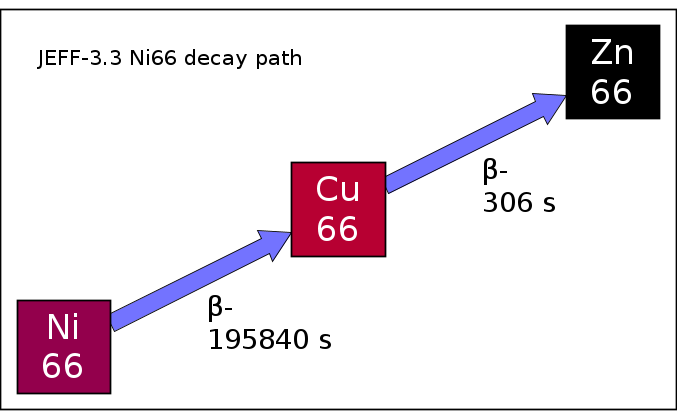
\includegraphics[width=.4\linewidth]{appendix/activity_equation/decay_paths/28ni66_decay.png}
		\captionsetup{font={it}}
		\caption{Decay path for Nickel-66 \cite{jeff311}}
		\label{fig:decayni66}
\end{figure}
\FloatBarrier

Nickel-66 beta decays to Copper-66 and then to Zinc-66.  The trial data are in table \ref{table:ni66trialdata}.  The \acrshort{rss} error between the numeric and analytic code in this decay chain over all five trials was $9.40 \times 10^{-2}$ and the total percentage error between the two was $1.52 \times 10^{-4}\%$.

\begin{table}[h]
\begin{center}
\begin{longtable}{c c c c c c c}
\hline\hline
 &  & Trial 1 & Trial 2 & Trial 3 & Trial 4 & Trial 5 \\
\hline\hline
${}^{66}_{28}Ni$ & $\omega$ & 
${0.0} \times 10^{0}$ & ${1.0} \times 10^{2}$ & ${0.0} \times 10^{0}$ &
${2.5} \times 10^{0}$ & ${2.5} \times 10^{0}$ \\
 & $n_{\text{start}}$ & 
${0.0} \times 10^{0}$ & ${0.0} \times 10^{0}$ & ${1.0} \times 10^{2}$ & 
${3.0} \times 10^{4}$ & ${3.0} \times 10^{4}$ \\
Numeric & $n_{\text{end}}$ & 
${0.0} \times 10^{0}$ & ${7.44391} \times 10^{6}$ & ${7.36534} \times 10^{1}$ & 
${2.08194} \times 10^{5}$ & ${2.08194} \times 10^{5}$ \\
Analytic & $n_{\text{end}}$ & 
${0.0} \times 10^{0}$ & ${7.44391} \times 10^{6}$ & ${7.36534} \times 10^{1}$ & 
${2.08194} \times 10^{5}$ & ${2.08194} \times 10^{5}$ \\
\hline
${}^{66}_{29}Cu$ & $\omega$ & 
${0.0} \times 10^{0}$ & ${0.0} \times 10^{0}$ & ${0.0} \times 10^{0}$ &
${0.0} \times 10^{0}$ & ${1.07} \times 10^{0}$ \\
 & $n_{\text{start}}$ & 
${0.0} \times 10^{0}$ & ${0.0} \times 10^{0}$ & ${0.0} \times 10^{0}$ &
${0.0} \times 10^{0}$ & ${1.0} \times 10^{3}$ \\
Numeric & $n_{\text{end}}$ & 
${0.0} \times 10^{0}$ & ${1.15802} \times 10^{4}$ & ${1.15264} \times 10^{-1}$ & 
${3.24085} \times 10^{2}$ & ${7.96452} \times 10^{2}$ \\
Analytic & $n_{\text{end}}$ & 
${0.0} \times 10^{0}$ & ${1.15802} \times 10^{4}$ & ${1.15264} \times 10^{-1}$ & 
${3.24085} \times 10^{2}$ & ${7.96452} \times 10^{2}$ \\
\hline
${}^{49}_{22}Ti$ & $\omega$ & 
${0.0} \times 10^{0}$ & ${0.0} \times 10^{0}$ & ${0.0} \times 10^{0}$ &
${0.0} \times 10^{0}$ & ${3.2} \times 10^{0}$ \\
 & $n_{\text{start}}$ & 
${0.0} \times 10^{0}$ & ${0.0} \times 10^{0}$ & ${0.0} \times 10^{0}$ &
${0.0} \times 10^{0}$ & ${2.0} \times 10^{4}$ \\
Numeric & $n_{\text{end}}$ & 
${0.0} \times 10^{0}$ & ${1.18451} \times 10^{6}$ & ${2.62314} \times 10^{1}$ & 
${3.74822} \times 10^{4}$ & ${4.26938} \times 10^{5}$ \\
Analytic & $n_{\text{end}}$ & 
${0.0} \times 10^{0}$ & ${1.18451} \times 10^{6}$ & ${2.62314} \times 10^{1}$ & 
${3.74822} \times 10^{4}$ & ${4.26938} \times 10^{5}$ \\
\hline\hline
\end{longtable}
\end{center}
\caption{Nickel-66 - numeric vs analytic calculated radioactivity}
\label{table:ni66trialdata}
\end{table}





\clearpage
\subsection{Caesium-125}

\FloatBarrier
\begin{figure}[!h]
\centering
		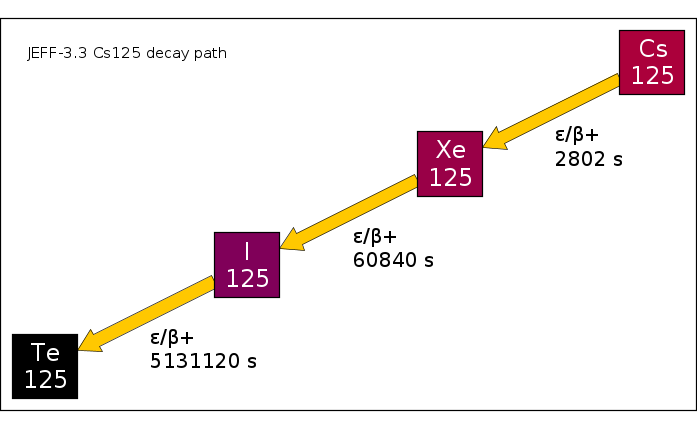
\includegraphics[width=.4\linewidth]{appendix/activity_equation/decay_paths/55cs125_decay.png}
		\captionsetup{font={it}}
		\caption{Decay path for Caesium-125 \cite{jeff311}}
		\label{fig:decaycs125}
\end{figure}
\FloatBarrier


The \acrshort{rss} error between the numeric and analytic code in this decay chain over all five trials was $6.42 \times 10^{-1}$ and the total percentage error between the two was $1.23 \times 10^{-3}\%$.

\begin{table}[h]
\begin{center}
\begin{longtable}{c c c c c c c}
\hline\hline
 &  & Trial 1 & Trial 2 & Trial 3 & Trial 4 & Trial 5 \\
\hline\hline
${}^{125}_{55}Cs$ & $\omega$ & 
${0.0} \times 10^{0}$ & ${1.0} \times 10^{2}$ & ${0.0} \times 10^{0}$ &
${5.0} \times 10^{1}$ & ${2.3} \times 10^{1}$ \\
 & $n_{\text{start}}$ & 
${0.0} \times 10^{0}$ & ${0.0} \times 10^{0}$ & ${1.0} \times 10^{2}$ & 
${2.0} \times 10^{5}$ & ${3.0} \times 10^{5}$ \\
Numeric & $n_{\text{end}}$ & 
${0.0} \times 10^{0}$ & ${4.0424} \times 10^{5}$ & ${5.2204} \times 10^{-8}$ & 
${2.0212} \times 10^{5}$ & ${9.2976} \times 10^{4}$ \\
Analytic & $n_{\text{end}}$ & 
${0.0} \times 10^{0}$ & ${4.0424} \times 10^{5}$ & ${5.2204} \times 10^{-8}$ & 
${2.0212} \times 10^{5}$ & ${9.2976} \times 10^{4}$ \\
\hline
${}^{125}_{54}Xe$ & $\omega$ & 
${0.0} \times 10^{0}$ & ${0.0} \times 10^{0}$ & ${0.0} \times 10^{0}$ &
${0.0} \times 10^{0}$ & ${5.4} \times 10^{1}$ \\
 & $n_{\text{start}}$ & 
${0.0} \times 10^{0}$ & ${0.0} \times 10^{0}$ & ${0.0} \times 10^{0}$ & 
${0.0} \times 10^{0}$ & ${2.0} \times 10^{2}$ \\
Numeric & $n_{\text{end}}$ & 
${0.0} \times 10^{0}$ & ${5.3391} \times 10^{6}$ & ${3.9172} \times 10^{1}$ & 
${2.7479} \times 10^{6}$ & ${4.3142} \times 10^{6}$ \\
Analytic & $n_{\text{end}}$ & 
${0.0} \times 10^{0}$ & ${5.3391} \times 10^{6}$ & ${3.9172} \times 10^{1}$ & 
${2.7479} \times 10^{6}$ & ${4.3142} \times 10^{6}$ \\
\hline$
{}^{125}_{53}I$ & $\omega$ & 
${0.0} \times 10^{0}$ & ${0.0} \times 10^{0}$ & ${0.0} \times 10^{0}$ &
${0.0} \times 10^{0}$ & ${2.1} \times 10^{1}$ \\
 & $n_{\text{start}}$ & 
${0.0} \times 10^{0}$ & ${0.0} \times 10^{0}$ & ${0.0} \times 10^{0}$ &
${0.0} \times 10^{0}$ & ${1.7} \times 10^{6}$ \\
Numeric & $n_{\text{end}}$ & 
${0.0} \times 10^{0}$ & ${2.8851} \times 10^{6}$ & ${6.0438} \times 10^{1}$ & 
${1.5634} \times 10^{6}$ & ${6.0191} \times 10^{6}$ \\
Analytic & $n_{\text{end}}$ & 
${0.0} \times 10^{0}$ & ${2.8851} \times 10^{6}$ & ${6.0438} \times 10^{1}$ & 
${1.5634} \times 10^{6}$ & ${6.0191} \times 10^{6}$ \\
\hline
${}^{125}_{52}Te$ & $\omega$ & 
${0.0} \times 10^{0}$ & ${0.0} \times 10^{0}$ & ${0.0} \times 10^{0}$ &
${0.0} \times 10^{0}$ & ${4.0} \times 10^{0}$ \\
 & $n_{\text{start}}$ & 
${0.0} \times 10^{0}$ & ${0.0} \times 10^{0}$ & ${0.0} \times 10^{0}$ &
${0.0} \times 10^{0}$ & ${5.0} \times 10^{4}$ \\
Numeric & $n_{\text{end}}$ & 
${0.0} \times 10^{0}$ & ${1.1544} \times 10^{4}$ & ${3.8975} \times 10^{-1}$ & 
${6.5513} \times 10^{3}$ & ${4.3678} \times 10^{5}$ \\
Analytic & $n_{\text{end}}$ & 
${0.0} \times 10^{0}$ & ${1.1544} \times 10^{4}$ & ${3.8975} \times 10^{-1}$ & 
${6.5513} \times 10^{3}$ & ${4.3678} \times 10^{5}$ \\
\hline\hline
\end{longtable}
\end{center}
\caption{Caesium-125 - numeric vs analytic calculated radioactivity}
\label{table:cs125trialdata}
\end{table}


\clearpage
\subsection{Bismuth-213}
\FloatBarrier

\begin{figure}[!h]
\centering
		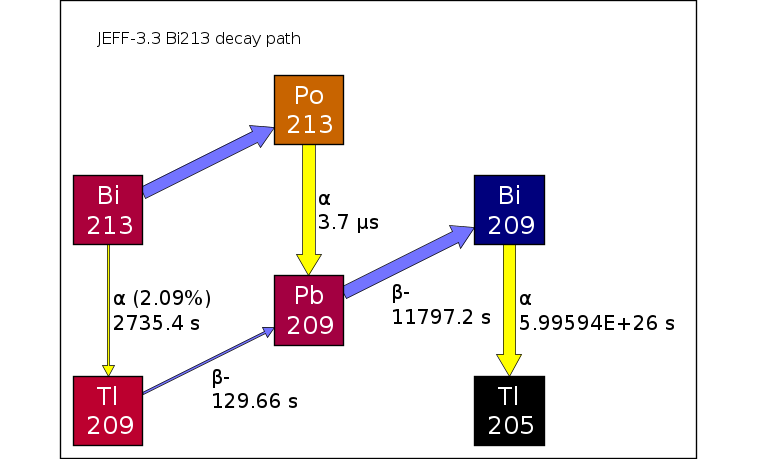
\includegraphics[width=.4\linewidth]{appendix/activity_equation/decay_paths/83bi213_decay.png}
		\captionsetup{font={it}}
		\caption{Decay path for Bismuth-213 \cite{jeff311}}
		\label{fig:decaybi213}
\end{figure}
\FloatBarrier

The previous decay examples have been straight chains with no branches, but Bismuth-213 is the first discussed in this section to have a branch.  There's approximately an 98\% chance that ${}^{213}_{83}Bi$ will decay to ${}^{213}_{83}Tl$ by alpha decay and just over 2\% chance that it will decay to ${}^{213}_{84}Po$ by beta decay.  These both go on to decay to ${}^{209}_{82}Pb$ that then undergoes beta decay to ${}^{209}_{83}Bi$.  There is another step in the chain (to the stable isotope ${}^{205}_{81}Tl$), but ${}^{209}_{83}Bi$ is observationally stable with an extremely long half life and the decay code terminates the chain at this point.

The \acrshort{rss} error between the numeric and analytic code in this decay chain over all five trials was $2.03 \times 10^{13}$.  This is large, but due mostly to the larger amounts used in this example.  The total percentage error between the two was $6.07 \times 10^{3}\%$ which is again large, but this is due to the numeric code and the short half life of Po-213 in comparison to the time step used.  Without the contribution of Po-213 the total percentage error between the two sets of results is just $2.37 \times 10^{-4}\%$.


\begin{table}[h]
\begin{center}
\begin{longtable}{c c c c c c c}
\hline\hline
 &  & Trial 1 & Trial 2 & Trial 3 & Trial 4 & Trial 5 \\
\hline\hline
${}^{213}_{83}Bi$ & $\omega$ & 
${0.0} \times 10^{0}$ & ${1.0} \times 10^{2}$ & ${0.0} \times 10^{0}$ &
${3.0} \times 10^{5}$ & ${3.0} \times 10^{5}$ \\
 & $n_{\text{start}}$ & 
${0.0} \times 10^{0}$ & ${0.0} \times 10^{0}$ & ${1.0} \times 10^{0}$ & 
${1.0} \times 10^{10}$ & ${1.0} \times 10^{10}$ \\
Numeric & $n_{\text{end}}$ & 
${0.0} \times 10^{0}$ & ${3.9463} \times 10^{5}$ & ${3.1024} \times 10^{-8}$ & 
${1.1839} \times 10^{9}$ & ${1.1839} \times 10^{9}$ \\
Analytic & $n_{\text{end}}$ & 
${0.0} \times 10^{0}$ & ${3.9463} \times 10^{5}$ & ${3.1024} \times 10^{-8}$ & 
${1.1839} \times 10^{9}$ & ${1.1839} \times 10^{9}$ \\
\hline$
{}^{213}_{84}Po$ & $\omega$ & 
${0.0} \times 10^{0}$ & ${0.0} \times 10^{0}$ & ${0.0} \times 10^{0}$ &
${0.0} \times 10^{0}$ & ${7.0} \times 10^{3}$ \\
 & $n_{\text{start}}$ & 
${0.0} \times 10^{0}$ & ${0.0} \times 10^{0}$ & ${0.0} \times 10^{0}$ &
${0.0} \times 10^{0}$ & ${2.0} \times 10^{7}$ \\
Numeric & $n_{\text{end}}$ & 
${0.0} \times 10^{0}$ & ${8.4594} \times 10^{-3}$ & ${6.6504} \times 10^{-16}$ & 
${2.5378} \times 10^{1}$ & ${2.5983} \times 10^{1}$ \\
Analytic & $n_{\text{end}}$ & 
${0.0} \times 10^{0}$ & ${5.2264} \times 10^{-4}$ & ${4.1088} \times 10^{-17}$ & 
${1.5679} \times 10^{0}$ & ${1.6053} \times 10^{0}$ \\
\hline
${}^{209}_{81}Tl$ & $\omega$ & 
${0.0} \times 10^{0}$ & ${0.0} \times 10^{0}$ & ${0.0} \times 10^{0}$ &
${0.0} \times 10^{0}$ & ${2.0} \times 10^{4}$ \\
 & $n_{\text{start}}$ & 
${0.0} \times 10^{0}$ & ${0.0} \times 10^{0}$ & ${0.0} \times 10^{0}$ &
${0.0} \times 10^{0}$ & ${2.0} \times 10^{6}$ \\
Numeric & $n_{\text{end}}$ & 
${0.0} \times 10^{0}$ & ${3.9096} \times 10^{2}$ & ${3.2265} \times 10^{-11}$ & 
${1.1729} \times 10^{6}$ & ${4.9141} \times 10^{6}$ \\
Analytic & $n_{\text{end}}$ & 
${0.0} \times 10^{0}$ & ${3.9096} \times 10^{2}$ & ${3.2265} \times 10^{-11}$ & 
${1.1729} \times 10^{6}$ & ${4.9141} \times 10^{6}$ \\
\hline
${}^{209}_{82}Pb$ & $\omega$ & 
${0.0} \times 10^{0}$ & ${0.0} \times 10^{0}$ & ${0.0} \times 10^{0}$ &
${0.0} \times 10^{0}$ & ${1.0} \times 10^{0}$ \\
 & $n_{\text{start}}$ & 
${0.0} \times 10^{0}$ & ${0.0} \times 10^{0}$ & ${0.0} \times 10^{0}$ &
${0.0} \times 10^{0}$ & ${1.0} \times 10^{7}$ \\
Numeric & $n_{\text{end}}$ & 
${0.0} \times 10^{0}$ & ${1.6881} \times 10^{6}$ & ${8.1281} \times 10^{-1}$ & 
${5.1457} \times 10^{9}$ & ${5.6026} \times 10^{9}$ \\
Analytic & $n_{\text{end}}$ & 
${0.0} \times 10^{0}$ & ${1.6881} \times 10^{6}$ & ${8.1281} \times 10^{-1}$ & 
${5.1457} \times 10^{9}$ & ${5.6026} \times 10^{9}$ \\
\hline
${}^{209}_{83}Bi$ & $\omega$ & 
${0.0} \times 10^{0}$ & ${0.0} \times 10^{0}$ & ${0.0} \times 10^{0}$ &
${0.0} \times 10^{0}$ & ${3.5} \times 10^{8}$ \\
 & $n_{\text{start}}$ & 
${0.0} \times 10^{0}$ & ${0.0} \times 10^{0}$ & ${0.0} \times 10^{0}$ &
${0.0} \times 10^{0}$ & ${1.0} \times 10^{6}$ \\
Numeric & $n_{\text{end}}$ & 
${0.0} \times 10^{0}$ & ${6.5568} \times 10^{6}$ & ${9.9187} \times 10^{1}$ & 
${2.9589} \times 10^{10}$ & ${3.0271} \times 10^{13}$ \\
Analytic & $n_{\text{end}}$ & 
${0.0} \times 10^{0}$ & ${6.5568} \times 10^{6}$ & ${9.9187} \times 10^{1}$ & 
${2.9589} \times 10^{10}$ & ${3.0271} \times 10^{13}$ \\
\hline
${}^{205}_{81}Tl$ & $\omega$ & 
${0.0} \times 10^{0}$ & ${0.0} \times 10^{0}$ & ${0.0} \times 10^{0}$ &
${0.0} \times 10^{0}$ & ${1.0} \times 10^{-10}$ \\
 & $n_{\text{start}}$ & 
${0.0} \times 10^{0}$ & ${0.0} \times 10^{0}$ & ${0.0} \times 10^{0}$ &
${0.0} \times 10^{0}$ & ${1.0} \times 10^{-10}$ \\
Numeric & $n_{\text{end}}$ & 
${0.0} \times 10^{0}$ & ${0.0} \times 10^{0}$ & ${0.0} \times 10^{0}$ & 
${0.0} \times 10^{0}$ & ${0.0} \times 10^{0}$ \\
Analytic & $n_{\text{end}}$ & 
${0.0} \times 10^{0}$ & ${0.0} \times 10^{0}$ & ${0.0} \times 10^{0}$ & 
${0.0} \times 10^{0}$ & ${0.0} \times 10^{0}$ \\
\hline\hline
\end{longtable}
\end{center}
\caption{Bismuth-213 - numeric vs analytic calculated radioactivity}
\label{table:bi213trialdata}
\end{table}




\clearpage
\subsection{Polonium-216}
\FloatBarrier

\begin{figure}[!h]
\centering
		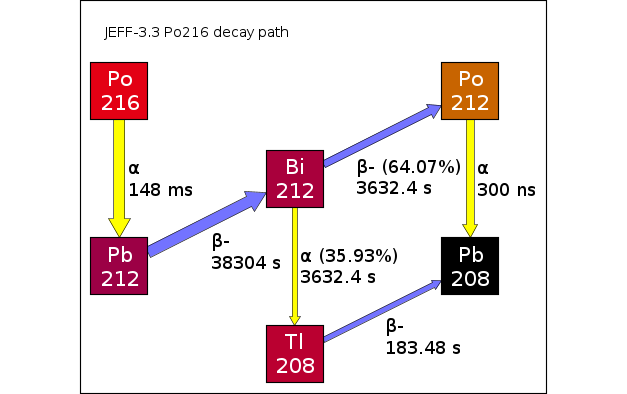
\includegraphics[width=.4\linewidth]{appendix/activity_equation/decay_paths/84po216_decay.png}
		\captionsetup{font={it}}
		\caption{Decay path for Bismuth-213 \cite{jeff311}}
		\label{fig:decaybi213}
\end{figure}
\FloatBarrier

The \acrshort{rss} error between the numeric and analytic code in this decay chain over all five trials was $3.85 \times 10^{1}$ and the total percentage error between the two was $7.94 \times 10^{4}\%$.  This large error was due to a short half life isotope (Po-212) and the comparatively long time step in the numeric solver.  Without this result, the agreement between numeric and analytic is $6.10 \times 10^{-2}\%$.

\begin{table}[h]
\begin{center}
\begin{longtable}{c c c c c c c}
\hline\hline
 &  & Trial 1 & Trial 2 & Trial 3 & Trial 4 & Trial 5 \\
\hline\hline
${}^{216}_{84}Po$ & $\omega$ & 
${0.0} \times 10^{0}$ & ${1.0} \times 10^{2}$ & ${0.0} \times 10^{0}$ &
${3.5} \times 10^{2}$ & ${2.0} \times 10^{-1}$ \\
 & $n_{\text{start}}$ & 
${0.0} \times 10^{0}$ & ${0.0} \times 10^{0}$ & ${1.0} \times 10^{2}$ & 
${5.0} \times 10^{4}$ & ${1.0} \times 10^{2}$ \\
Numeric & $n_{\text{end}}$ & 
${0.0} \times 10^{0}$ & ${2.13562} \times 10^{1}$ & ${0.0} \times 10^{0}$ & 
${7.47467} \times 10^{1}$ & ${4.27124} \times 10^{-2}$ \\
Analytic & $n_{\text{end}}$ & 
${0.0} \times 10^{0}$ & ${2.13519} \times 10^{1}$ & ${0.0} \times 10^{0}$ & 
${7.47316} \times 10^{1}$ & ${4.27038} \times 10^{-2}$ \\
\hline$
{}^{212}_{82}Pb$ & $\omega$ & 
${0.0} \times 10^{0}$ & ${0.0} \times 10^{0}$ & ${0.0} \times 10^{0}$ &
${0.0} \times 10^{0}$ & ${2.0} \times 10^{-1}$ \\
 & $n_{\text{start}}$ & 
${0.0} \times 10^{0}$ & ${0.0} \times 10^{0}$ & ${0.0} \times 10^{0}$ &
${0.0} \times 10^{0}$ & ${5.0} \times 10^{0}$ \\
Numeric & $n_{\text{end}}$ & 
${0.0} \times 10^{0}$ & ${4.36891} \times 10^{6}$ & ${2.09405} \times 10^{1}$ & 
${1.53016} \times 10^{7}$ & ${1.31287} \times 10^{4}$ \\
Analytic & $n_{\text{end}}$ & 
${0.0} \times 10^{0}$ & ${4.36891} \times 10^{6}$ & ${2.09405} \times 10^{1}$ & 
${1.53017} \times 10^{7}$ & ${1.31287} \times 10^{4}$ \\
\hline
${}^{212}_{83}Bi$ & $\omega$ & 
${0.0} \times 10^{0}$ & ${0.0} \times 10^{0}$ & ${0.0} \times 10^{0}$ &
${0.0} \times 10^{0}$ & ${7.0} \times 10^{-2}$ \\
 & $n_{\text{start}}$ & 
${0.0} \times 10^{0}$ & ${0.0} \times 10^{0}$ & ${0.0} \times 10^{0}$ &
${0.0} \times 10^{0}$ & ${1.50} \times 10^{1}$ \\
Numeric & $n_{\text{end}}$ & 
${0.0} \times 10^{0}$ & ${4.02810} \times 10^{5}$ & ${2.19385} \times 10^{0}$ & 
${1.41093} \times 10^{6}$ & ${1.57757} \times 10^{3}$ \\
Analytic & $n_{\text{end}}$ & 
${0.0} \times 10^{0}$ & ${4.02810} \times 10^{5}$ & ${2.19385} \times 10^{0}$ & 
${1.41093} \times 10^{6}$ & ${1.57757} \times 10^{3}$ \\
\hline
${}^{208}_{81}Tl$ & $\omega$ & 
${0.0} \times 10^{0}$ & ${0.0} \times 10^{0}$ & ${0.0} \times 10^{0}$ &
${0.0} \times 10^{0}$ & ${5.0} \times 10^{-3}$ \\
 & $n_{\text{start}}$ & 
${0.0} \times 10^{0}$ & ${0.0} \times 10^{0}$ & ${0.0} \times 10^{0}$ &
${0.0} \times 10^{0}$ & ${1.0} \times 10^{1}$ \\
Numeric & $n_{\text{end}}$ & 
${0.0} \times 10^{0}$ & ${7.30001} \times 10^{3}$ & ${4.00077} \times 10^{-2}$ & 
${2.55700} \times 10^{4}$ & ${1.83923} \times 10^{-5}$ \\
Analytic & $n_{\text{end}}$ & 
${0.0} \times 10^{0}$ & ${} \times 10^{}$ & ${} \times 10^{}$ & 
${} \times 10^{}$ & ${} \times 10^{}$ \\
\hline
${}^{212}_{84}Po$ & $\omega$ & 
${0.0} \times 10^{0}$ & ${0.0} \times 10^{0}$ & ${0.0} \times 10^{0}$ &
${0.0} \times 10^{0}$ & ${2.0} \times 10^{-2}$ \\
 & $n_{\text{start}}$ & 
${0.0} \times 10^{0}$ & ${0.0} \times 10^{0}$ & ${0.0} \times 10^{0}$ &
${0.0} \times 10^{0}$ & ${1.7} \times 10^{1}$ \\
Numeric & $n_{\text{end}}$ & 
${0.0} \times 10^{0}$ & ${4.25501} \times 10^{-3}$ & ${2.31743} \times 10^{-8}$ & 
${1.49041} \times 10^{-2}$ & ${1.83923} \times 10^{-5}$ \\
Analytic & $n_{\text{end}}$ & 
${0.0} \times 10^{0}$ & ${2.13149} \times 10^{-5}$ & ${1.16088} \times 10^{-10}$ & 
${7.46601} \times 10^{-5}$ & ${9.21338} \times 10^{-8}$ \\
\hline
${}^{208}_{82}Pb$ & $\omega$ & 
${0.0} \times 10^{0}$ & ${0.0} \times 10^{0}$ & ${0.0} \times 10^{0}$ &
${0.0} \times 10^{0}$ & ${1.0} \times 10^{-2}$ \\
 & $n_{\text{start}}$ & 
${0.0} \times 10^{0}$ & ${0.0} \times 10^{0}$ & ${0.0} \times 10^{0}$ &
${0.0} \times 10^{0}$ & ${3.0} \times 10^{2}$ \\
Numeric & $n_{\text{end}}$ & 
${0.0} \times 10^{0}$ & ${3.86096} \times 10^{6}$ & ${7.68257} \times 10^{1}$ & 
${1.35518} \times 10^{7}$ & ${2.07028} \times 10^{4}$ \\
Analytic & $n_{\text{end}}$ & 
${0.0} \times 10^{0}$ & ${3.86096} \times 10^{6}$ & ${7.68257} \times 10^{1}$ & 
${1.35518} \times 10^{7}$ & ${2.07028} \times 10^{4}$ \\
\hline\hline
\end{longtable}
\end{center}
\caption{Polonium-216 - numeric vs analytic calculated radioactivity}
\label{table:po216trialdata}
\end{table}








\clearpage
\subsection{Radon-218}
\FloatBarrier

\begin{figure}[!h]
\centering
		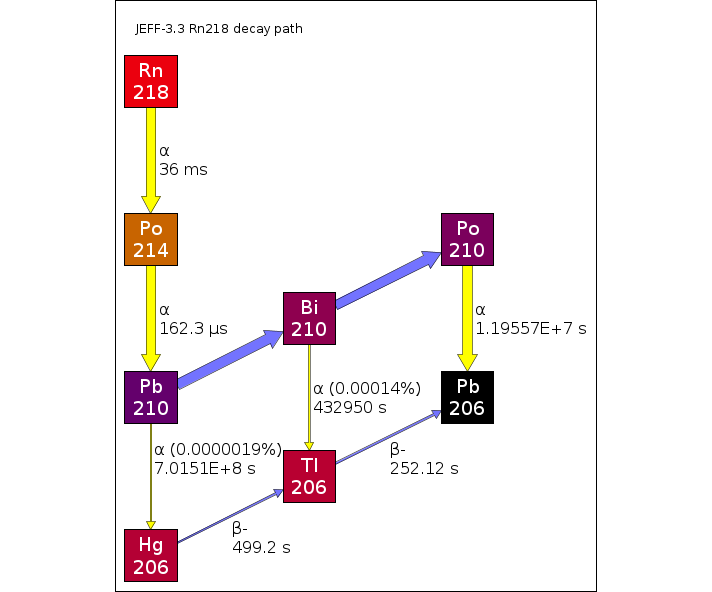
\includegraphics[width=.4\linewidth]{appendix/activity_equation/decay_paths/86rn218_decay.png}
		\captionsetup{font={it}}
		\caption{Decay path for Bismuth-213 \cite{jeff311}}
		\label{fig:decayrn218}
\end{figure}
\FloatBarrier


The \acrshort{rss} error between the numeric and analytic code in this decay chain over all five trials was $1.73 \times 10^{3}$ and the total percentage error between the two was $5.93 \times 10^{1}\%$.  However, if the short half life isotope Po-214 is excluded, the error is just $5.15 \times 10^{-1}\%$.


\begin{table}[h]
\begin{center}
\begin{longtable}{c c c c c c c}
\hline\hline
 &  & Trial 1 & Trial 2 & Trial 3 & Trial 4 & Trial 5 \\
\hline\hline
${}^{218}_{86}Rn$ & $\omega$ & 
${0.0} \times 10^{0}$ & ${1.0000} \times 10^{0}$ & ${0.0000} \times 10^{0}$ &
${3.5} \times 10^{2}$ & ${3.5000} \times 10^{2}$ \\
 & $n_{\text{start}}$ & 
${0.0000} \times 10^{0}$ & ${0.0000} \times 10^{0}$ & ${1.0000} \times 10^{0}$ & 
${5.0000} \times 10^{4}$ & ${5.0000} \times 10^{4}$ \\
Numeric & $n_{\text{end}}$ & 
${0.0000} \times 10^{0}$ & ${5.1980} \times 10^{0}$ & ${0.0000} \times 10^{0}$ & 
${1.8193} \times 10^{1}$ & ${1.8193} \times 10^{1}$ \\
Analytic & $n_{\text{end}}$ & 
${0.0000} \times 10^{0}$ & ${5.1937} \times 10^{0}$ & ${0.0000} \times 10^{0}$ & 
${1.8178} \times 10^{1}$ & ${1.8178} \times 10^{1}$ \\
\hline
${}^{214}_{84}Po$ & $\omega$ & 
${0.0000} \times 10^{0}$ & ${0.0000} \times 10^{0}$ & ${0.0000} \times 10^{0}$ &
${0.0000} \times 10^{0}$ & ${7.0000} \times 10^{1}$ \\
 & $n_{\text{start}}$ & 
${0.0000} \times 10^{0}$ & ${0.0000} \times 10^{0}$ & ${0.0000} \times 10^{0}$ &
${0.0000} \times 10^{0}$ & ${1.0000} \times 10^{3}$ \\
Numeric & $n_{\text{end}}$ & 
${0.0000} \times 10^{0}$ & ${2.8000} \times 10^{-2}$ & ${0.0000} \times 10^{0}$ & 
${9.8000} \times 10^{-2}$ & ${1.1760} \times 10^{-1}$ \\
Analytic & $n_{\text{end}}$ & 
${0.0000} \times 10^{0}$ & ${2.3415} \times 10^{-2}$ & ${0.0000} \times 10^{0}$ & 
${8.1952} \times 10^{-2}$ & ${9.8343} \times 10^{-1}$ \\
\hline
${}^{210}_{82}Pb$ & $\omega$ & 
${0.0000} \times 10^{0}$ & ${0.0000} \times 10^{0}$ & ${0.0000} \times 10^{0}$ &
${0.0000} \times 10^{0}$ & ${1.0000} \times 10^{3}$ \\
 & $n_{\text{start}}$ & 
${0.0000} \times 10^{0}$ & ${0.0000} \times 10^{0}$ & ${0.0000} \times 10^{0}$ &
${0.0000} \times 10^{0}$ & ${1.2000} \times 10^{2}$ \\
Numeric & $n_{\text{end}}$ & 
${0.0000} \times 10^{0}$ & ${8.6396} \times 10^{6}$ & ${9.9991} \times 10^{1}$ & 
${3.0289} \times 10^{7}$ & ${1.2273} \times 10^{8}$ \\
Analytic & $n_{\text{end}}$ & 
${0.00000} \times 10^{0}$ & ${8.6396} \times 10^{6}$ & ${9.9991} \times 10^{1}$ & 
${3.0289} \times 10^{7}$ & ${1.2273} \times 10^{8}$ \\
\hline
${}^{206}_{80}Hg$ & $\omega$ & 
${0.0000} \times 10^{0}$ & ${0.0000} \times 10^{0}$ & ${0.0000} \times 10^{0}$ &
${0.0000} \times 10^{0}$ & ${1.7000} \times 10^{1}$ \\
 & $n_{\text{start}}$ & 
${0.0000} \times 10^{0}$ & ${0.0000} \times 10^{0}$ & ${0.0000} \times 10^{0}$ &
${0.0000} \times 10^{0}$ & ${7.0000} \times 10^{2}$ \\
Numeric & $n_{\text{end}}$ & 
${0.0000} \times 10^{0}$ & ${1.1585} \times 10^{-7}$ & ${1.3520} \times 10^{-12}$ & 
${4.0614} \times 10^{-7}$ & ${1.2243} \times 10^{4}$ \\
Analytic & $n_{\text{end}}$ & 
${0.00000} \times 10^{0}$ & ${1.1584} \times 10^{-7}$ & ${1.3519} \times 10^{-12}$ & 
${4.0611} \times 10^{-7}$ & ${1.2243} \times 10^{4}$ \\
\hline
${}^{210}_{83}Bi$ & $\omega$ & 
${0.0000} \times 10^{0}$ & ${0.0000} \times 10^{0}$ & ${0.0000} \times 10^{0}$ &
${0.0000} \times 10^{0}$ & ${2.3000} \times 10^{1}$ \\
 & $n_{\text{start}}$ & 
${0.0000} \times 10^{0}$ & ${0.0000} \times 10^{0}$ & ${0.0000} \times 10^{0}$ &
${0.0000} \times 10^{0}$ & ${4.1000} \times 10^{1}$ \\
Numeric & $n_{\text{end}}$ & 
${0.0000} \times 10^{0}$ & ${3.5238} \times 10^{2}$ & ${7.9731} \times 10^{-3}$ & 
${1.2373} \times 10^{3}$ & ${1.8609} \times 10^{-6}$ \\
Analytic & $n_{\text{end}}$ & 
${0.00000} \times 10^{0}$ & ${3.5236} \times 10^{2}$ & ${7.9725} \times 10^{-3}$ & 
${1.2372} \times 10^{3}$ & ${1.8609} \times 10^{6}$ \\
\hline
${}^{206}_{81}Tl$ & $\omega$ & 
${0.0000} \times 10^{0}$ & ${0.0000} \times 10^{0}$ & ${0.0000} \times 10^{0}$ &
${0.0000} \times 10^{0}$ & ${8.1000} \times 10^{1}$ \\
 & $n_{\text{start}}$ & 
${0.0000} \times 10^{0}$ & ${0.0000} \times 10^{0}$ & ${0.0000} \times 10^{0}$ &
${0.0000} \times 10^{0}$ & ${5.0000} \times 10^{2}$ \\
Numeric & $n_{\text{end}}$ & 
${0.0000} \times 10^{0}$ & ${3.4319} \times 10^{-7}$ & ${7.1575} \times 10^{-12}$ & 
${1.2047} \times 10^{-6}$ & ${3.5646} \times 10^{4}$ \\
Analytic & $n_{\text{end}}$ & 
${0.00000} \times 10^{0}$ & ${3.4316} \times 10^{-7}$ & ${7.1570} \times 10^{-12}$ & 
${1.2046} \times 10^{-6}$ & ${3.5646} \times 10^{4}$ \\
\hline
${}^{210}_{84}Po$ & $\omega$ & 
${0.0000} \times 10^{0}$ & ${0.0000} \times 10^{0}$ & ${0.0000} \times 10^{0}$ &
${0.0000} \times 10^{0}$ & ${5.2000} \times 10^{2}$ \\
 & $n_{\text{start}}$ & 
${0.0000} \times 10^{0}$ & ${0.0000} \times 10^{0}$ & ${0.0000} \times 10^{0}$ &
${0.0000} \times 10^{0}$ & ${1.5000} \times 10^{3}$ \\
Numeric & $n_{\text{end}}$ & 
${0.0000} \times 10^{0}$ & ${1.6413} \times 10^{1}$ & ${5.6320} \times 10^{-4}$ & 
${5.7726} \times 10^{1}$ & ${4.4948} \times 10^{7}$ \\
Analytic & $n_{\text{end}}$ & 
${0.00000} \times 10^{0}$ & ${1.6411} \times 10^{1}$ & ${5.6316} \times 10^{-4}$ & 
${5.7722} \times 10^{1}$ & ${4.4948} \times 10^{7}$ \\
\hline
${}^{206}_{82}Pb$ & $\omega$ & 
${0.0000} \times 10^{0}$ & ${0.0000} \times 10^{0}$ & ${0.0000} \times 10^{0}$ &
${0.0000} \times 10^{0}$ & ${1.0000} \times 10^{3}$ \\
 & $n_{\text{start}}$ & 
${0.0000} \times 10^{0}$ & ${0.0000} \times 10^{0}$ & ${0.0000} \times 10^{0}$ &
${0.0000} \times 10^{0}$ & ${1.0000} \times 10^{4}$ \\
Numeric & $n_{\text{end}}$ & 
${0.0000} \times 10^{0}$ & ${2.0729} \times 10^{-2}$ & ${9.5248} \times 10^{-7}$ & 
${7.3026} \times 10^{-2}$ & ${9.4943} \times 10^{7}$ \\
Analytic & $n_{\text{end}}$ & 
${0.00000} \times 10^{0}$ & ${2.0747} \times 10^{-2}$ & ${9.5242} \times 10^{-7}$ & 
${7.3089} \times 10^{-2}$ & ${9.4943} \times 10^{7}$ \\
\hline\hline
\end{longtable}
\end{center}
\caption{Radon-218 - numeric vs analytic calculated radioactivity}
\label{table:rn218trialdata}
\end{table}
































\begin{comment}
\begin{table}[h]
\begin{center}
\begin{longtable}{c c c c c c c}
\hline\hline
 &  & Trial 1 & Trial 2 & Trial 3 & Trial 4 & Trial 5 \\
\hline\hline
${}^{49}_{24}Cr$ & $\omega$ & 
${0.0} \times 10^{0}$ & ${} \times 10^{}$ & ${} \times 10^{}$ &
${} \times 10^{}$ & ${} \times 10^{}$ \\
 & $n_{\text{start}}$ & 
${0.0} \times 10^{0}$ & ${} \times 10^{}$ & ${} \times 10^{}$ & 
${} \times 10^{}$ & ${} \times 10^{}$ \\
Numeric & $n_{\text{end}}$ & 
${0.0} \times 10^{0}$ & ${} \times 10^{}$ & ${} \times 10^{}$ & 
${} \times 10^{}$ & ${} \times 10^{}$ \\
Analytic & $n_{\text{end}}$ & 
${0.0} \times 10^{0}$ & ${} \times 10^{}$ & ${} \times 10^{}$ & 
${} \times 10^{}$ & ${} \times 10^{}$ \\
\hline$
{}^{49}_{23}V$ & $\omega$ & 
${0.0} \times 10^{0}$ & ${0.0} \times 10^{0}$ & ${0.0} \times 10^{0}$ &
${0.0} \times 10^{0}$ & ${} \times 10^{}$ \\
 & $n_{\text{start}}$ & 
${0.0} \times 10^{0}$ & ${0.0} \times 10^{0}$ & ${0.0} \times 10^{0}$ &
${0.0} \times 10^{0}$ & ${} \times 10^{}$ \\
Numeric & $n_{\text{end}}$ & 
${0.0} \times 10^{0}$ & ${} \times 10^{}$ & ${} \times 10^{}$ & 
${} \times 10^{}$ & ${} \times 10^{}$ \\
Analytic & $n_{\text{end}}$ & 
${0.0} \times 10^{0}$ & ${} \times 10^{}$ & ${} \times 10^{}$ & 
${} \times 10^{}$ & ${} \times 10^{}$ \\
\hline
${}^{49}_{23}V$ & $\omega$ & 
${0.0} \times 10^{0}$ & ${0.0} \times 10^{0}$ & ${0.0} \times 10^{0}$ &
${0.0} \times 10^{0}$ & ${} \times 10^{}$ \\
 & $n_{\text{start}}$ & 
${0.0} \times 10^{0}$ & ${0.0} \times 10^{0}$ & ${0.0} \times 10^{0}$ &
${0.0} \times 10^{0}$ & ${} \times 10^{}$ \\
Numeric & $n_{\text{end}}$ & 
${0.0} \times 10^{0}$ & ${} \times 10^{}$ & ${} \times 10^{}$ & 
${} \times 10^{}$ & ${} \times 10^{}$ \\
Analytic & $n_{\text{end}}$ & 
${0.0} \times 10^{0}$ & ${} \times 10^{}$ & ${} \times 10^{}$ & 
${} \times 10^{}$ & ${} \times 10^{}$ \\
\hline\hline
\end{longtable}
\end{center}
\caption{}
\label{table:template}
\end{table}
\end{comment}

